% CSC 300: Professional Responsibilities Dr. Clark Turner

% Two Column Format
\documentclass[11pt]{article}
%this allows us to specify sections to be single or multi column so that things
%like title page and table of contents are single column
\usepackage{multicol}
\usepackage{indentfirst}
\usepackage[english]{babel}
\usepackage[utf8x]{inputenc}
\usepackage{setspace} 
\usepackage{verbatim}
\usepackage{url}
\usepackage{pdfpages}
\usepackage{graphicx}
\usepackage{breakurl}

%%% PAGE DIMENSIONS
\usepackage{geometry} % to change the page dimensions 
\geometry{letterpaper}

\begin{document}

\title{\vfill Peek-a-Boo \\ \large Tor vs Iran}
\author{ 
  By Orion Miller\vspace{10pt} \\
  CSC 300: Professional Responsibilities \vspace{10pt} \\
  Dr. Clark Turner\vspace{10pt} \\
}
%\date{October 22, 2010} %Or use \today for today's Date
\date{\today}

\maketitle

\vfill  %in combinaion with \newpage this forces the abstract to the bottom of
\begin{abstract} 
  DA DA DA
\end{abstract}

\thispagestyle{empty} %remove page number from title page 

\newpage

\thispagestyle{empty}  %Remove page number from TOC 

\tableofcontents

\newpage

%end the 1 column format


%start 2 column format
\begin{multicols}{2}
%Start numbering first page of content as page 1
\setcounter{page}{1}
%%%%%%%%%%%%%%%%%%%%
%%% Known Facts  %%%
%%%%%%%%%%%%%%%%%%%%
\section{Facts} 

\subsection{Iran's Presidential Election}

In Iran, the sparks of political unrest began to fly in the summer of 2009.
Friction started with the highly anticipated outcome of the Iran's race for
presidency. Elections took place on June 12th. To the surprise of many, Mahmoud
Ahmadinajad won with a lanslide victory of well above 60\% of the vote
\footnote{The Interior Ministry was the part of the Iranian government that
tallied the votes of the election}  \cite{TheIranianVote,
IranianElectionResultsByProvince} , making this Ahmadinjad's second term as the
President of Iran.

\subsection{The Response}

Iranian citizens and many others were outraged with the results of the election.
Laura Secor from the New Yorker, succinctly sumed up the voice of Iranian
dissidents by stating 
\begin{quotation} 
  ``there can be no question that on June 12, 2009, the Iranian presidential 
  election was stolen.'' \cite{TheIranianVote}
\end{quotation} 
Citizens swiftly began to vocalize their opinions.

\subsection{Protests Begin}

Protests began on June 13 and picked up force not only offline but online as
well. By the fifth day of protests, hundreds of thousands of demonstrators took to
the streets of Tehran in opposition of the election's outcome
\cite{IranProtestsFifthDayOfUnrest}. At the same time, ``the
Twitterverse\footnote{Twitterverse is a name referring everything relating to
the social network Twitter.} exploded with tweets from people who weren't having
it, both in English and in Farsi.'' \cite{WhyTwitterIsTheMedium}

\subsection{Iran Tries to Stop the Protests}

Iran's government tried to douse out the dissent. They sent
Revolutionary Gaurds into the streets, cut off the Internet, and shut down
cell-phone communications. \cite{TheIranianVote} The government didn't stop
there, they began to specifically arresting, ``at least 500 activists,
opposition figures, journalists.'' \cite{IranProtestsFifthDayOfUnrest} The
Iranian government didn't stop at just arresting protesters they made certain
locations of protest a threat to life. The government publicly announced that
the police had orders to shoot anyone approaching the Interior Ministry.
\cite{TheIranianVote} Online, the government filtered their internet traffic and
for periods of times blocked social networks like Twitter \footnote{Twitter is a
microblogging service were anyone can read, write, and share messages, up to 140
characters long.  \cite{WhatIsTwitter}}.  \cite{IranBlocksFacebookTwitter}

%%TWITTER FOOTNOTE - add source from "What is Twitter, a social network or a
%% News media
\subsection{The Role of Internet}

The Internet provided a medium for political discorse where traditional media
was failing. Blogs and social networks, especially Twitter, began to prove
themselves invaluabale.  Where traditional means of sharing information such as
newspapers were breaking down, online sources of information were playing a
vital role during the protests by providing a global, uncensored, and near
real-time means of news, communication, and organization.  In Iran, ``while the
front pages of Iranian newspapers were full of blank space where censors had
whited-out news stories, Twitter was delivering information from street level,
in real time.'' \cite{WhyTwitterIsTheMedium}

\subsection{Citizens use Tor to Bypass Censorship}

With the government filtering out vital lifelines of information and means of
organization, citizens began to find alternatives to connect to Twitter.
\cite{FindingWayAroundIranianCensorship} One of the tools that proved useful was
Tor.

\subsection{What is Tor}

Tor\footnote{In this paper when the term `Tor' is used it will refer to the
software.} is software that connects and participates in the Tor network that
provides users a means way of connecting with websites that is encrypted and
anonymous. In short, The Tor Project publicizes that, ``The Tor software is a
program you can run on your computer that helps keep you safe on the
Internet.''\cite{Tor:FAQ} 

\subsection{Iran Blocks Tor}

Two years after, Iran is still under the same regime of Ahmadinajad.  On
September 14, 2011 the Iranian government added a filter rule to their firewall
and blocked Tor traffic despite Tors main focused intent on preventing such
things from ever happening. \cite{IranBlocksTorSameDayFix}  Later that day the
Tor project released a patch which circumvent Iran's firewall filters and
suggested users of Tor to upgrade to version Tor 0.2.2.33 or Tor
0.2.3.4-alpha.\cite{IranBlocksTorSameDayFix}

%%%%%%%%%%%%%%%%%%%%%%%%%
%%% Research Question %%%
%%%%%%%%%%%%%%%%%%%%%%%%%
\section{Research Question} 
Was it ethical for the Tor project to release a same day patch specifically
enabling Iranians to bypass Iran's firewall when the government explicitely
filtered Tor traffic starting September 14, 2011?

\subsection{Importance of Question}

This research question is important because in essence it is asking wether The
Tor Project should be involved in Iran's political discorse and is it acting in
an ethical manor. Most importnatly Iranian dissidents are being jailed and some
cases killed.\cite{IranBloggersDeath} Tor and its network could provide a safe
and private means for discorse and dissent to exist.


%%%%%%%%%%%%%%%%%%%%%%%%%
%%% Extant Arguments from External Sources %%%
%%%%%%%%%%%%%%%%%%%%%%%%%
\section{Extant Arguments} 

There have been little to no published articles specifically finding the Tor's
patch in response to Iran's Tor block ethical or not. In general arguments for
or against Tor revolve around what it allows people to do rather than the
software itself.

\subsection{Arguments Against Tor}

The Iranian government has and currently firmly believes that it is necessary to
censor the Internet traffic coming in and out of the country. They have
announced that they feel it is right to censor the Internet because they feel
they need to stamp out ``immoral and illegal''
content.\cite{CensorshipFearsRise} It is true that immoral and illegal content
exists on the Internet and Tor can be used to facilitate child porn and
drugs.\cite{Tor:ChildPorn, Tor:SilkRoad} We can safely assume that the Iranian
government finds Tor to be unethical because it can allow people to bypass what
they consider to be necessary Internet filters that the Iranian government has
specifically blocked Tor.\cite{IranBlocksTorSameDayFix}

\subsection{Arguments For Tor}

The arguments for Tor stem from the feeling that anonymity online is fundamental
for people to communicate freely without the fear of repercussion or
retribution.\cite{Tor:ArgumentForAppelbaum} People arguing for Tor do
acknowledge that it can be used for evil but Jacob Appelbaum, an Advocate,
Security Researcher, and Developer for The Tor Project, feels that
\begin{quotation} 
  
  ``yes, it is possible that [Tor] could be misused. But I believe the problem
  of bad speech is not solved by censoring speech or by tracking people down and
  harming them, but rather it is solved with more
  speech.''\cite{Tor:ArgumentForAppelbaum}

\end{quotation}
Despite Tor's negative possible uses it gives its users, 
"anonymity [, which] is not only a core value of the digital age, it is a vital
underpinning of the right to free speech."\cite{TorCreatesSaferInternet}




\subsection{Arguments Summary}

Tor brings up the debated issue of wether people should have anonymity and if so
how much. On one hand it can be a tool to facilitate malicious behavior in the
world, or as a tool to subvert the rules imposing a nations moral framework. On
the other hand it is argued that even though it can be used for bad on whole it
is  better that good people are empowered with this tool so they can exercise
their fundamental rights of privacy and freedom of speech.

%%%%%%%%%%%%%%%%
%%% Analysis %%%
%%%%%%%%%%%%%%%%
\section{Analysis}

For or us analyze the research question and see if The Tor
Project was ethical we need to utilize an ethical system as a framework
to guide the analysis and and as a foundation to determine what is and is
not ethical. This paper will use the Association for Computing
Machinery's\footnote{On ACM's `About' webpage it statest that, ``ACM is widely recognized as the premier membership
  organization for computing professionals, delivering resources that advance
  computing as a science and a profession; enable professional development; and
promote policies and research that benefit society.''\cite{ACM:About}}
Software Engineering Code of ethics (SE Code). Before we begin analysis under this code of
ethics we need to examine and determine if the SE Code of ethics applies to
the domain of the research question.

\subsection{Why the SE Code of Ethics Applies} 

The Software Engineering Code of Ethics states that, ``Software engineers are
those who contribute by direct participation or by teaching, to the analysis,
specification, design, development, certification, maintenance and testing of
software systems.'' \cite{SE:CodeOfEthics} The Tor Project is a 501(c)(3)
non-profit based in the United States that makes internet anonymity
software.\cite{Tor:FAQ, Tor:CorePeople} Their Mission Statement states that,

\begin{quotation}
  ``the Corporation is organized and shall be operated exclusively for scientific,
  charitable and educational purposes ... to develop, improve and distribute
  free, publicly available tools and \textbf{programs} that promote free speech, free
expression, civic engagement and privacy rights online''\footnote{ The entirity
of The Tor Project's missions statement can be found in Appendix
\ref{Tor:MissionStatement}} \cite{TOR:Sponsorship} 
\end{quotation}

Looking at the the keyword porgrams within The Tor Project's mission statement
we need to make sure it would be considered a software system under the SE
Code's preamble. The Oxford Dictionary defines software as, ``the programs and other operating
information used by a computer.''\cite{defn:Software} Using the Oxford
Dictionary's defintion it equates software with programs used by a computer.
Taking Oxford's definition and applying it to Tor's Mission Statement we would
get, ``... to develop, improve and distrube free, publicly available tools and
\textbf{software} that promote ...''
Because the Tor Project develops, and distributes software, this means they, ``contribute by
direct participation ...  to the analysis, specification, design, development,
... , maintenance and testing of software systems'' and thus are Software
Engineers, meaning The Tor Project falls under the requirements of the Software
Engineering Code of Ethics.\cite{Tor:FAQ, Tor:Overview} 


\subsection{SE Code 1.07} 

By the the Tor project releasing a patch on September 14, the same day that Iran
added filters to block out Tor traffic in their firewall, meant that The Tor
Project was directly responding to the current events of Iran.

\fbox{
  \parbox{0.8\linewidth}{
    1.07. Consider issues ...  and \textbf{other factors} that can
    \textbf{diminish access} to the \textbf{benefits} of \textbf{software}. 
    \cite{SE:CodeOfEthics}
}}
\newline

To bring this ethical argument into the domain of the research question a few
modifications to the code need to made. The phrase \textbf{other factors} in
this case is \textbf{Iran's firewall block of Tor}. The phrase \textbf{diminish
access} in this case \textbf{prevents access}. The word \textbf{benefits} in
this case is the \textbf{uncensored Internet}. The word \textbf{software} in
this case is \textbf{Tor}.

\subsubsection{Applying SE Code 1.07 to the Tor Project}

\fbox{ 
  \parbox{0.8\linewidth}{ 
    1.07. Consider the issue of ... \textbf{Iran's firewall block of Tor} that 
    \textbf{preventents access} to the \textbf{uncensored Internet} from 
    \textbf{Tor}.
    \cite{SE:CodeOfEthics}
}}
\newline

Our question now can be broken down into three parts. First, how did Tor
circumvent Iran's firewall? Second, how did the Tor software patch affect
uncensored Internet access?  Lastly, was Tor ethical under SE Code 1.07?

\subsubsection{Iran's Firewall}
Before we investigate how Tor bypasses Iran's firewall or the considerations and
effects of the Tor patch we need to examine how Iran's firewall works.

\paragraph{Internet Service}

All of the Internet service in Iran is controlled by Data Communications of Iran
(DCI). \cite{FindingWayAroundIranianCensorship} In addition to DCI's monopoly on
Iran's Internet, it is mainly owned by the Iranian government.
\cite{FindingWayAroundIranianCensorship, DCI:Articles} This gives DCI and the
Iranian government, the ability to throttle the total amount of data that enters
and leaves the country, specify what websites are accessable by defining filter
rules on their routers, and the ability to turn off the Internet all together.
\cite{FindingWayAroundIranianCensorship}

\paragraph{Censorship} 

It is one thing for the Iranian government have control over Iran's
Internet, but is it on within their power to actually censor and monitor DCI's
Internet users? In 2009 DCI, for a brief period took down the entire Internet in 
Iran. \cite{FindingWayAroundIranianCensorship} Specific websites such a
Facebook, Youtube, Twitter, and Google had been blocked from access.
\cite{FindingWayAroundIranianCensorship, IransElectronicCurtain} The blocking of
these sites does not just block what Iran's government may consider illegitimate
use of such websites, it  blocks legitimate use of these sites by Iranians and
for those whom they may be trying to communicate with using these sites under
Iran's ethical framework. The Iranian government also took measures to filter
SSL traffic and specifically the Tor network.  \cite{Tor:IranPartiallyBlocksSSL,
IranBlocksTorSameDayFix} Blocking SSL traffic may appear just a means for the
government to filter and monitor Internet traffic but it has larger
implications. Encrypting network traffic is fundmental for Internet users to
protect themselves from malicious people gathering sensative information like
passwords, banking informations, and medical information. Given Iran's power
over DCI and their past and current actions they have taken to exercise that
power demonstrates, that they want to control the information and communications
of its people, especially Iranian dissidents.


\subsubsection{How did Tor circumvent Iran's firewall?}

Now that we have an understanding what the Iranian firewall is capable of it is
important to examing how Tor is capable of bypassing it.

\paragraph{How Tor Works}
\label{HowTorWorks}
We will examine how Tor works by analogy of sending and receiving mail 
exchagned between people. 
\footnote{The reason for an explanation with analogy is to avoid the prequisite
  knowledge of computing and computer networks. For additional information on how 
  Tor works visit Appendix \ref{Tor:HowTorWorks} or head to
  \url{https://www.torproject.org/about/overview.html.en#overview} and
\url{http://freehaven.net/anonbib/}
}

We will define a \textbf{Tor node} as a \textbf{person}, \textbf{data} as a
\textbf{letter}, \textbf{encryption} as an \textbf{envelope}, and
\textbf{directory server} as an \textbf{address book}.  Tor in this analogy works
by following the steps as follows. Bill wants to send a letter his friend Alice
while preventing anyone from reading his message or discover what his address is.  Bill
is smart so he devises plan. He looks through his address book and finds three
friends and their addresses.  These three friends (Zulu, Yankee, X-ray)
have agreed to forward any message that they receive to the
specified address on the envelope. Bill chooses a path for hist letter to take take from one friend
to the next to reach Alice. In this analogy it will go from Zulu to Yankee to
X-ray and finally Alice. Before Bill does anything else he a devises a unique
means for each envelope to only be able to be opened by the recipient of that
letter and exchanges that information to said recipient.  Then he takes his letter addressed to Alice from Bob and then
puts it in the first envelope addressed From Yankee to X-ray.  Then Bob puts first
envelope into a second enevelope addressed from Zulu to Yankee.  Finally puts the second
envelope inside a third envelope addressed from Bill to Zulu.  Then he sends
this tripple wrapped letter off to Zulu.  As each friend receives their envelope addressed to them
they open it and send it off to the friend it is stated on the envelope.  This
way, no one along the path from Bill to Alice, except for Bill, knows the source address of
Bill and the destination address of Alice at the same time.  The
only ones who can read the message is X-ray and Alice. This is basically how Tor
software works. It should be noted that putting an envelope around the original letter
before it's encased by the enevelopes for Zulu, Yankee, and X-ray is out of
the scope of the Tor protocol.

\paragraph{Dousing the Firewall}

Continuing from the analogy above, we can analyze how Bill (i.e an Iranian
dissident) could use this technique to subvert the access controls specified by
the Iranan firewall. Iranian dicidents being able to use Tor to connect to the
Tor network would connect other Tor nodes and set up a path. Tor could be
specified to make sur the last node in the path, the exit node, is outside Iran.
\cite{Tor:SpecificExitNode, Tor:FAQ} The data being sent across the designated
path would reach its end address (e.g.  Twitter, Facebook) and Iran's firewall
would not be able to censor or monitor that data. The Iranian government
wouldn't be able to censor what websites the Iranian dissident wants to access
since the firewall doesn't know the end address. The Iranian government wouldn't
be able to monitor Iranian dissidents traffic since the data on the path in Iran
is encrypted. However, Iran could and has blocked Tor traffic
itself.

\subsubsection{Did The Tor Project consider the release of the Tor patch?} 

At this point we can examine the consideration The Tor Project's made for the
release of Tor 0.2.2.33 and 0.2.3.4-alpha. There was little to no data found on
a consideration to release this specific patch. The next best thing we
can do is to infer a consideration of this patch by looking at information that
plausibly would factor into the consideration of releasing this software. To do
this we shall look at the technical and social topics surrounding this release
that could have impacted the decision process of release.

\paragraph{Quality}

The Tor Project takes Tor and the Tor network very seriously and critically.
They openly admit that their software is not perfect by any means. Despite this,
there have been considerable amounts of academic and government research on
anonymity networks and revision of the Tor project. \cite{Tor:ResearchPapers}
Tor's source code and design documents are fully open to the public to review
and scrutinize, it is event stated on The Tor Project's `Research Ideas' web-page
that, ``we need people to attack the system, quantify defenses, etc.''
\cite{Tor:ResearchIdeas, Tor:2011} Since open source code and design documents
might not be enough  they provide a growing repository of tools to take metrics
and attack the Tor network. \cite{Tor:ResearchHome} ``DEFINE SECURE SOFTWARE''.
It appears that The Tor Project does its best to meet this definition of
security for their users.  

\paragraph{Tor Is Blocked}

On September 14th, 2011 the Iranian government added a filter to their `firewall'
that blocked Tor traffic. They were able to do this by checking Tor's expiration
time of SSL \footnote{SSL (Secure Socket Layer) - Is a cryptographic protocol to
hide inormation.} session certificates \footnote{session certificate - is a
means of authenticating an SSL connection.} . This was possible because at the
time, Tor's SSL session certificates were set to expire after two hours where normal SSL
certificats would usually last a year or longer. For a short period of time this
effectively blocked Iranian dicidents who used Tor from receiving its benefits
of an uncensored Internet. \cite{IranBlocksTorSameDayFix}

\paragraph{The Patch} 

The Tor Project was able to fix this within the same day by changing the
certificates to have a, ``larger expiration time ..., so our certs have more
plausible expiry times.'' \cite{IranBlocksTorSameDayFix} \footnote{There appeared to be
nothing written about considering technical and social issues specifically
related to the release of Tor 0.2.2.33 and 0.2.3.4-alpha.}  However it was
implied in the blog post \textit{Iran blocks Tor; Tor releases same-day fix}
that the patch was a simple fix. \cite{IranBlocksTorSameDayFix} From this it
would be fair to assume that this change in the software did not drastically
change the robustness of the software from the prior version and therefore did
not put any users in any new danger.

\paragraph{Social Issues}

With the Iranian government killing, jailing, and generally harrasing Iranian
dissidents, it is a good idea that Iranian dissidents make it as hard as
possible to prevent themselves from falling subject to the regime of their
government.  Tor, while not perfect, does its best to give its users the benefit
of anonymity and an uncensored Internet. It is not unreasonable to conclude that
The Tor Project believes that Iranian dissidents are better off using The Tor
Project's software than not to use any anonymity software at all. In regards to
the release of the patch, it was probably logical to The Tor Project that the
software be patched as timely as possible and released for use.

\paragraph{Consideration}

From what we have established, it is fair to say that we can infer an
approximate idea of what The Tor Project was considering during this patch.
Since the Tor patch was considered a minimal change to the current robust code
base, there was little to no fear about the update patch causing a negative
technical issue and resulting in diminished asccess to the uncensored Internet.
In regards to the social issues possibly preventing the release of the patch,
The Tor Project felt that Iranian dissidents would be better off with the
release of the patch.


%\subsubsection{How did the Tor software patch affect uncensored Internet
%access?}

\subsubsection{Was Tor ethical under SE Code 1.07?}

%\section{Rawlsian Justice Principle Analysis}
%%can another ethical system apply

%%preamble ''public interest''
%%the Rawlsian Justice principle gives us another means of critical analysis of
%%what would the public interest be in this case

%\subsection{Applying Rawlsian}

%%citizens are the majority has the most to gain and government who has most power
%%dissimination of knowledge
%% allows them to question the ethical framwework that Iran Govt. tries to
%%   impose
%% 
%% freedom of press statistics
%% happiness & freedom of press statistics


\subsection{SE Code 3.03}

\fbox{ 
  \parbox{0.8\linewidth}{ 
    3.03. ... Address \textbf{ethical}, \textbf{economic}, (and)
    \textbf{cultural}, ... issues related to \textbf{work projects}.
    \cite{SE:CodeOfEthics}
}}
\newline

To bring this ethical argument into the domain of The Tor Project aiding Iranian
dicicdents, a few modifications to the code need to be made. The
\textbf{ethical} issue in this case is the issue of \textbf{freedom of
expression}. The \textbf{economic} issues in this case is the issue of
\textbf{Tor software's financial cost} (i.e. the financial cost on the users of
the software). The \textbf{cultural} issues in this case is refering to
\textbf{Iran's oppression of online dissidents}. The phrase \textbf{work
projects} in this case referes to \textbf{Tor software}.

%The Tor software is a \textbf{work project} that has identified, defined, and
%addressed is to directly project directly concerned its software with the one of
%its hopes to provide, ``Journalists use Tor to communicate more safely with
%whistleblowers and dissidents.

\subsubsection{Applying SE Code 3.03 to the Tor Project}

\fbox{
  \parbox{0.8\linewidth}{
    3.03. ... Address \textbf{freedom of expression},
    \textbf{Tor's financial cost}, (and) \textbf{Iran's oppression of dissidents},
    ... issues related to \textbf{Tor software}.  
    \cite{SE:CodeOfEthics}
}}
\newline

Our question now can be broken up into four parts. First, does Tor software
promote freedom of expression in Iran? Second, what is the financial cost for
Tor users?  Third, does Tor software mitigate Iran's oppression of dissidents?
Lastly, is Tor ethical under SE code 3.03.

\subsubsection{The state of Freedom of Expression in Iran}
Before we investigate wether Tor addresses freedom of expression in Iran we need
to examine what the current sate of freedom of expression is in Iran. 

\paragraph{Freedom of Expression Definition}

For analysis of this paper we will need define `freedom of expression' somewhat
broadly. It will be synonymsous with freedom of expression, speech, opinion, and
press.  This needs to be the case because of the nature that the Internet,
social networks and blogs have played in this case. The foundation of this
redefintion of `freedom of expression' stems from 
\begin{quotation} 
  A free press is defined not only by the media's freedom to say what they want
  but also by media consumers' freedom to get the information they need.
  \cite{PublicAttitudeTowardFreedomPress, ComplexRoadToHappiness}
\end{quotation}

In addition, we need note that the terms `media' and `media consumers' from the
quote above in our case need to include the people who post content and read
content from blogs, Twitter, social networks, and other forms of communication
online since the importance of these forms of medium have played in Iran but in
addition to that for example Twitter has been shown to show accurate news
events.  \cite{Twitter:BreakingNewsDetection, Twitter:IdentificationLiveEvents,
Twitter:MeasuringInfluence}


\paragraph{Universal Declaration of Human Rights}

We should examine Iran's relationship to the United Nations to temper our
analysis of their actions in how they censor their citizens. 

(!!!!!how it applies to under 3.03 code entry and how it is means to guide goals
of the state.)

Iran is and has been a member of the United Nations since 1945.
\cite{UN:IranBecameMember, UN:IranActiveMember} Under the United Nations `The
Universal Declaration of Human Rights' it states that ``Member States
\footnote{Member States are countries that are members of the United Nations}
have pledged themselves to achieve, in co-operation with the United Nations, the
promotion of universal respect for and observance of human rights and
fundamental freedoms.''\cite{UniversalDeclerationOfHumanRights}. It appears
that, under this pledge Member States should strive to uphold `The Universal
Declaration of Human Rights' preamble and articles. Article 19 states

\begin{quotation} 
  Everyone has the right to freedom of opinion and expression;
  this right include freedom to hold opinions without interference and to seek,
  receive and impart information and ideas through any media and regardless of
  frontiers.  \cite{UniversalDeclerationOfHumanRights}
\end{quotation}

(put in mutual knowledge form Steve Pinker and possibly the mission statement
again - it should be clear that the Tor project is trying to ensure this to all
Iranian users and that the Iranian government appears to be trying to prevent
freedom of speech)


\paragraph{Iranian Government's Censorship}


\subparagraph{Internet Police}

%statistics on websites shutdown
%considered how bad it is
%reasons they claim they shutdown
%reasons why other people believe it is being shut down

\paragraph{Monitorship}

%Iran's Firewall could be considered not to be just passive access controls on
%the Internet but active response to what is being posted and discussed on the
%Internet. Iran's Internet Police, FATA....

%current setup ability to censor and monitor, internet police that monitors
%internet uses and, case examples of censoring communications, SSL traffic,
%faceboook, youtube, and this paper - tor

\subsubsection{Does Tor promote freedom of expression?}

It is important to take note of not only the actions that is taken, or in this
case what Tor software has done and provides users, but the driving ethos behind
the project by the projects maintainers, The Tor Project.

\paragraph{Tor Projects's Ethos}

The organization that actively maintains Tor takes their software and mission
very seriously. It can be seen in The Tor Project's Mission Statement as in
Appendix \ref{Tor:MissionStatement} or more succintcly from their website
stating that,


\begin{quotation} 
  
  ``The Tor project is based on the belief that anonymity is not just a good
  idea some of the time — it is a requirement for a free and functioning
  society.''\cite{Tor:Users}

\end{quotation}


\paragraph{Tor and Free Speech}

Tor is created such that anonymity is not just some policy but implemented by
design. This anonymity allows users to have unrestricted access to the internet.
The other benefits of the software prevent anyone along the path to a server
from knowing the source and destination at the same time. These properties of
Tor make it a lot harder for third parties like the Iranian government to filter
and monitor network traffic of Tor users.

The Tor project has even been given The Free Software Foundation Award of 2010
for
\begin{quotation}Tor has enabled roughly 36 million people around the world to
  experience freedom of access and expression on the Internet while keeping them
  in control of their privacy and anonymity. Its network has proved pivotal in
  dissident movements in both Iran and more recently
Egypt.\cite{FreeSoftwareAwards} \end{quotation}

The Electronic Frontier Foundation (EFF) has taken it upon themselves to
endorse Tor. Under an EFF article titled `Surveillance Self-Defense' lists Tor
as a tool that can help you, ``protect the confidentiality of your
communications.''\cite{EFF:Tor} The Tor network requires the participation
of members of the network to create a more usable network. The EFF created `The
EFF Tor Challenge' to help support this network by having people volunteer and
hosting a Tor relay.\cite{EFF:TorChallenge} The goal was 500 relays and as of 
now 549 relays have been put up.\cite{EFF:TorChallenge}

Tor, with its anonymity by design and support from organizations like the EFF,
allow for Iranian dissidents to communicate freely. Tor removes the restrictions
that the Iranian government's firewall imposes and allows users to freely access
any website. Tor also removes the ability of the Iranian government to monitor
users, thus allowing them to freely associate and communicate with whom they
wish. 

(mutual knowledge quote Free Software award)

\subsubsection{What is the financial cost of Tor?}

We should examine the financial costs of Tor not only in the direct cost of the
software but it's indirect costs by being open-source.\footnote{This section
  will only examine a topical and broad analysis of financial issues regarding
  Iranian dissidents since a full analysis of the financial state of the average
Iranian dissident and those who use Tor probably could be an entire paper in it
itself.}

\paragraph{Tor in Regards to Beer}

To download and use Tor and the Tor network does not cost the user anything. By
making Tor free it does not discriminate on those who can `use' and those who
`cannot use' the software. 

It is fair to assume that some dissidents in Iran may not have had the money to
afford Tor if did cost anything. With Tor financial barrier removed and the
possible legitemate concerns of Iranian dissidents who may not be able to afford
Tor with a pricetag alleviated maximizes the number of dissidents using Tor.

\paragraph{Tor in Regards to Speech}
(help protesters in iran - run a tor relay)

Tor is `open source', which means anyone can ``[redistribute] and use in source
and binary forms, with or without modification, [is] permitted provided that''
Tor's 3-clause BSD license conditions are met. \footnote{Tor's full license can
be found in Appendix \ref{Tor:License}} \cite{BSD:3-ClauseLicense,
TOR:Download, TOR:BSD-License} 

By Tor being distributed as `open source' source code enable some inherent
qualities. It allows the source code for open review, which allows for anyone to
check for design or implementation flaws in the source code. In regards to this
case it allows Iranian dissidents to directly or by proxy check for flaws in
code so they can trust that Tor actually provides anonymity from the Iranian
government when they use Tor. This freedom also allows for anyone to modify the
code to the Tor Project, making it possible to modify the code to meet specific
or local issues. For Iranian dissidents this means that if ther was unique
censorship tools or modifications to the Internet within Iran they would have a
code base to operate from to modify the code to their local issue.  Indirectly,
Tor being `open source' makes it financially beneficial to Iranian dissidents.

\subsubsection{The State of Physical Oppression of Dissidents}
Before we investigate wether Tor addresses physical oppression of dissidents in
Iran, we need to examine what the current sate of physical oppression is.
\footnote{We will begin examining Iran's state of oppression with the beginning
of protests in response to Iran's 2009 presidential elections because this
appears origin of what is relevant to this paper.}

\paragraph{Death}

``Why is it that in our country political prisoners go to jail vertically but return
horizontally?'', Iranian MP, Ahmed Bakhshayes, asked the Iranian Parliament on
November 14, 2012.\cite{IranBloggersDeath} The Iranian government has been
responding to political dissidence by putting people to death. In the past ten
years at least eighteen people have died in while imprisoned by the Iranian
government, including the Iranian-Canadian photographer Zahra Kazemi, student
activist Amir Javadifar, a journalist Hoda Saber, and most recently a 35 year
old blogger, Sattar Beheshti. \cite{IranBloggersDeath}

%specific blogger killed
%addressed other bloggers jailed and killed

\subsubsection{Does Tor software mitigate Iran's physical oppression of
dissidents?}

Let us call a spade a spade, Tor is not a `silver bullet' for the physical
oppression going on in Iran. It however does have privacy by design. This does
make it much more challenging for the Iranian government to censor and monitor
Iranian dissidents. By Tor empowering Iranian dissidents to communicate in
privacy and journal events and opinions of Iranian current affairs, it prevents
the Iranian government from correlating the vocalized opinions it disagrees with
and revealing who are saying them. This veil of secrecy is what indirectly helps
Iranian dissidents from physical oppression.

% talk about tor hiding anonymity
% doesn't protect end-to-end
% if someone posts there name on an article Tor cannot protect against them
% talk about how it does make it more challenging for traffic analaysis
% no node can know about other nodes

\subsubsection{Was Tor ethical under SE code 3.03?}

%%%%%%%%%%%%%%%%%%
%%% Conclusion %%%
%%%%%%%%%%%%%%%%%%
\section{Conclusion} 


Roger Dingledine, during a talk about Tor last year stated that, ``it should not
be up to me how [Iran] \footnote{This quote originally said China however it could
  apply to any country so it was changed to fit the domain of this
paper.} changes, we write tools to let people all around the world change the
world in the way they think their world needs to change.'' \cite{Tor:28c3} Under
both of these tenents of the SE Code, we can conclude that The Tor Project was
ethical in releasing a same day patch enabling Iranians to bypass Iran's
firewall when the government explicitely filtered Tor traffic starting September
14, 2011.


%end the two column format
\end{multicols} \newpage

\appendix

\section{Tor's License}
\label{Tor:License}
\verbatiminput{appendix/TOR-LICENSE.txt}

\section{The Tor Project's Mission Statement}
\label{Tor:MissionStatement}

\verbatiminput{appendix/mission-statement.txt}

\section{Basics of How Tor Works}
\label{Tor:HowTorWorks}

\begin{center}
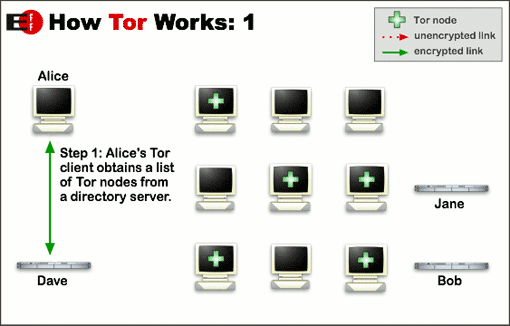
\includegraphics[natwidth=510bp,natheight=326bp,width= 0.7\linewidth]{appendix/htw1.png}
\end{center}
\verbatiminput{appendix/htw1.txt}

\begin{center}
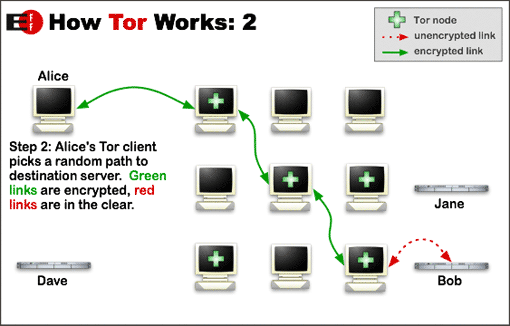
\includegraphics[natwidth=510bp,natheight=326bp,width= 0.7\linewidth]{appendix/htw2.png}
\end{center}
\verbatiminput{appendix/htw2.txt}

\begin{center}
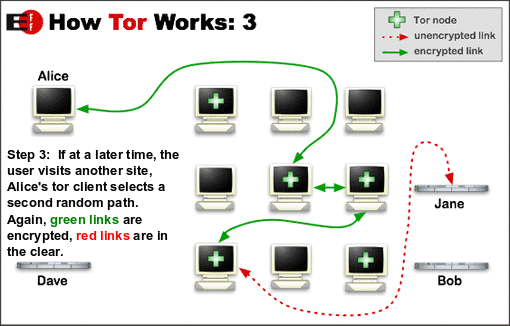
\includegraphics[natwidth=510bp,natheight=326bp,width= 0.7\linewidth]{appendix/htw3.png}
\end{center}

\newpage

%cite all the references from the bibtex you haven't explicitly cited
\nocite{*}

\bibliographystyle{IEEEannot}

\bibliography{texreport}

\end{document}
